\section{The User Interface}
\label{sec:UserInterface}
This section explores the user interface of the plugin. When the plugin is loaded and opened, the user is met with figure~\ref{fig:EasyInsertDevice}. This is the Device tab of EasyInsert and from here it is possible to select a device listed and load it into the WorkCell by pressing the Load button. Upon pressing Load, the user is prompted with a dialog window where the user can specify options about the loaded device. Figure~\ref{fig:loadDialog} is the exact dialog window the user would see after selecting a device and pressing the load button. The user can now give the device a unique name, select a frame that the device should be on and specify the configurations such as displacement and rotation. A user can now select e.g. a fanuc robot arm, as the one on figure~\ref{fig:FANUCLRM200}, and insert it. Afterwards the user can then select another device, let's say some kind of hand device, and now insert that device on the end frame of the fanuc. The hand device now acts as the end effector of the fanuc, which only took a few clicks to set up. 

\begin{figure}[h] % 3 figures of the tabs
        \begin{subfigure}[b]{0.32\textwidth}
                \centering
                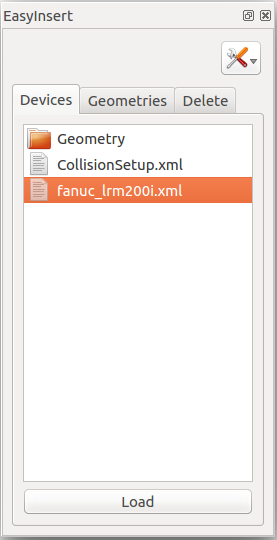
\includegraphics[width=.95\linewidth]{Figures/EasyInsertDevice.png}
  				\caption{Devices}
 				\label{fig:EasyInsertDevice}
        \end{subfigure}%
        \begin{subfigure}[b]{0.32\textwidth}
                \centering
                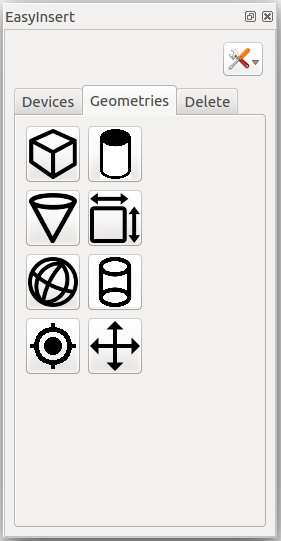
\includegraphics[width=.95\linewidth]{Figures/EasyInsertGeo.png}
  				\caption{Geometries}
  				\label{fig:EasyInsertGeo}
        \end{subfigure}%
        \begin{subfigure}[b]{0.32\textwidth}
                \centering
                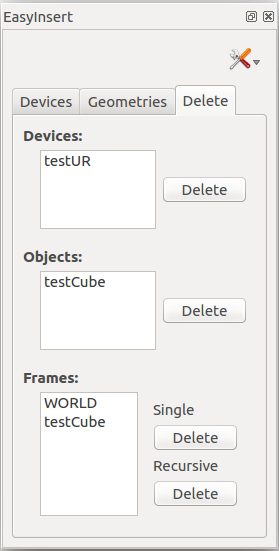
\includegraphics[width=.95\linewidth]{Figures/EasyInsertDelete.png}
  				\caption{Delete}
  				\label{fig:EasyInsertDelete}
        \end{subfigure}%
        \caption{The three tabs a user can interact with in the plugin. In Devices it is possible to select and load a device. In Geometries the user can click an icon (representing a geometry) which then prompts a dialog window with options regarding the insertion of said geometry. In Delete a user can select either a Device, Object or Frame to delete it.}\label{fig:EasyInsertTabs}
\end{figure}

It should be noted, that the first time EasyInsert is loaded and opened, the device tab shows the root content of the operating system. Thus the user needs to change the path of the list shown in the Device tab to a path containing any desired devices. In the right top corner of the plugin is a tool bar button (the only button in the tool bar so far) called settings. Clicking this button and choosing Libraries will prompt the user with the dialog window on Figure~\ref{fig:settingsDialog}. The user can here see what path is used and change it with the [...] button. The [...] button shows a new dialog window where the user can navigate his/her OS and specify the path that should be shown in the device tab.\\

\begin{figure}[h] % 3 figures of dialog windows
     \centering
     \begin{subfigure}[b]{0.45\textwidth}
	  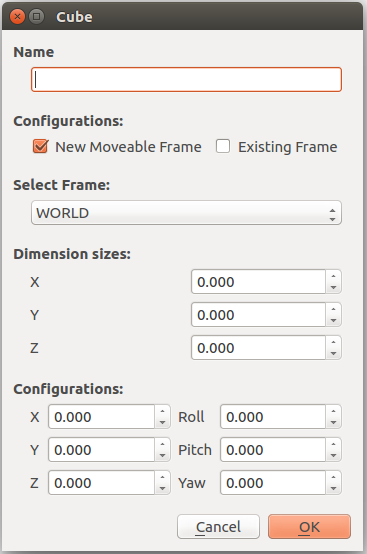
\includegraphics[scale=0.7]{Figures/EasyInsertCubeDialog.png}
       \caption{Cube insertion dialog window}\label{fig:cubeDialog}
     \end{subfigure}
     \hfill
     \begin{minipage}[b]{0.45\textwidth}
       \begin{subfigure}[b]{\linewidth}
	    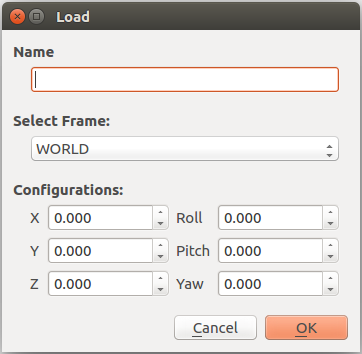
\includegraphics[scale=0.7]{Figures/EasyInsertLoadDialog.png}
         \caption{Device insertion dialog window}\label{fig:loadDialog}
       \end{subfigure}\\[\baselineskip]
       \begin{subfigure}[b]{\linewidth}
	    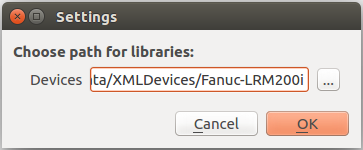
\includegraphics[scale=0.7]{Figures/settingsDialogWindow.png}
         \caption{Settings of device path dialog window}\label{fig:settingsDialog}
       \end{subfigure}
     \end{minipage}
     \caption{Three, out of many, dialog windows the user can experience and interact with when using EasyInsert.}\label{fig:EasyInsertDialogs}
\end{figure}

The Geometries tab shows a grid of icons, see figure~\ref{fig:EasyInsertGeo}. These icons represent either geometric primitives or frames that can be inserted into the WorkCell. Currently there are the following objects in the geometric tab, from top row to bottom:
\begin{enumerate*}[font={\color{red!50!black}\bfseries}]
\item Cube.
\item Cylinder.
\item Cone.
\item Plane.
\item Sphere.
\item Tube.
\item Fixed frame.
\item Movable frame.
\end{enumerate*}
These icons are all buttons the user can click, and after a click has occurred a dialog window appears with options regarding the insertion of said geometry. When the user hovers over a button in the Geometries tab, a tool tip identifying the icon appears, telling the user what sort of object it is. Figure~\ref{fig:cubeDialog} is the dialog window prompted when clicking the cube icon, and as seen, the user can specify a name for the geometry, select a reference frame and set the displacement and rotation configurations, just like when inserting a device. Though for a geometric primitive, like the cube, the user can also specify the dimensions of the geometric figure. The user can also specify whether the primitive should create a movable frame to associate the object with, or if the user want to use an existing frame.\\

The delete tab, as seen on figure~\ref{fig:EasyInsertDelete}, is a tab where the user can select a device, object or a frame and press either the Single Delete or Recursive Delete button to remove said item from the WorkCell. The Devices list, shown in the delete tab, shows a device name. This means that when the user deletes a device, the frames associated with that device are now "free", i.e. the device property is deleted, but the frames and objects are still in the WorkCell. These object and frames will now show up in the Object list and the Frames list of the delete tab, and the user can now remove the frames and objects from the WorkCell. The Object list of the delete tab only deletes objects, but if the user selects a frame from the Frame list and deletes it with either the Single Delete or Recursive Delete, all objects associated with that frame will also be deleted. Single Delete will only delete the selected frame, and if that frame has children, then the user will be noticed and the deletion is cancelled. Recursive Delete deletes the frame and all children of said frame. It should be noted that there are various problems with the frame delete functionalities, certain scenarios will cause a segmentation fault (properly a rogue pointer somewhere) in the program because of different reasons. These issues will be further discussed in section~\ref{sec:eiProblems}.